\documentclass[12pt]{article}

\usepackage{amssymb}
\usepackage{amsmath}
\usepackage{bm}
\usepackage{color}
\usepackage{float}
\usepackage{graphicx}
\usepackage{mathtools}
\usepackage[none]{hyphenat}
\usepackage{indentfirst}
\usepackage[labelfont=bf]{caption}
\usepackage[left=2.5cm,right=2.5cm, top=2.5cm,bottom=2.5cm]{geometry}
\usepackage{tcolorbox}
\usepackage{lineno}
\usepackage{setspace}
\DeclarePairedDelimiter\ceil{\lceil}{\rceil}

\usepackage[authoryear]{natbib}
\usepackage{hyperref}
\usepackage{yhmath}

\usepackage{dsfont}
\usepackage{mathtools}
\usepackage{soul}

\overfullrule 5pt

%\doublespacing

\usepackage{lipsum}

%\usepackage{adjustbox}
\usepackage{lscape}
\usepackage{afterpage}

\makeatletter
\renewcommand{\maketitle}{\bgroup\setlength{\parindent}{0pt}
\begin{flushleft}
\textbf{\@title}

  \@author
\end{flushleft}\egroup
}
\makeatother

\begin{document}

\linenumbers

\title{A Bayesian Model of the DNA Barcode Gap}

\author{Jarrett D. Phillips$^{1, 2*}$ (ORCID: 0000-0001-8390-386X)  \\
\textit{$^1$School of Computer Science, University of Guelph, Guelph, ON., Canada, N1G2W1} \\ \textit{$^2$Department of Integrative Biology, University of Guelph, Guelph, ON., Canada, N1G2W1} }

\date{}

\maketitle

\vspace{2mm}

\noindent \textbf{*Corresponding Author}: Jarrett D. Phillips$^{1}$

\noindent \textbf{Email Address}: jphill01@uoguelph.ca

\noindent \textbf{Running Title}: Bayesian inference for DNA barcode gap estimation

\newpage

\begin{abstract}

A simple statistical model of the DNA barcode gap is outlined. Specifically, \\ accuracy of recently introduced nonparametric metrics, inspired by coalescent theory, to characterize the extent of proportional overlap/separation in maximum and minimum pairwise genetic distances within and among species, respectively, is explored in both frequentist and Bayesian contexts. The empirical cumulative distribution function (ECDF) is utilized to estimate probabilities associated with positively skewed extreme tail distribution quantiles bounded on the closed unit interval [0, 1] based on a \\ straightforward binomial distance overlap count. Using R and Stan, the proposed maximum likelihood estimators and Bayesian model are demonstrated on cytochrome $b$ (CYTB) gene sequences from two \textit{Agabus} diving beetle species exhibiting limits in the extent of representative taxonomic sampling. MCMC simulations show much estimation uncertainty in parameter estimates given highly skewed posteriors, \\ particularly when specimen sample sizes for target species are small. Findings highlight the promise of the Bayesian approach using a conjugate beta prior for reliable posterior uncertainty estimation when available data are sparse. Obtained results can shed light on foundational and applied research questions concerning DNA-based specimen identification and species delineation for studies in evolutionary biology and ecology, as well as biodiversity conservation and management, of wide-ranging taxa.

\end{abstract}

\textbf{Keywords}: Bayesian/frequentist inference, DNA barcoding, intraspecific genetic \\ distance, interspecific genetic distance, specimen identification, species discovery

\vspace{2mm}

\section{Introduction}

The routine use of DNA sequences to support broad microevolutionary and \\ macroevolutionary hypotheses concerning processes like gene flow and speciation in diverse and spatially-distributed taxonomic lineages such as birds, fishes, insects, and arachnids took flight in the late 1980s \citep{avise1987intraspecific}. However, the application of molecular genomic data to applied fields like biodiversity forensics, conservation, and management came later (\textit{e.g.}, Forensically Informative Nucleotide Sequencing (FINS); \citet{bartlett1992fins}). Since its inception over 20 years ago, DNA barcoding \citep{hebert2003biological, hebert2003barcoding} has emerged as a robust method of specimen identification and species delimitation across myriad Eukaryotic groups which have been sequenced at short, standardized gene regions like the haploid cytochrome $c$ oxidase subunit I (5'-COI) mitochondrial locus for animals. However, the success of the approach, particularly for regulatory and forensic applications, depends crucially on two important factors: (1) the availability of high-quality specimen records found in public reference sequence databases such as the Barcode of Life Data Systems (BOLD; http://www.barcodinglife.org) \citep{ratnasingham2007bold} and GenBank (https://www.ncbi.nlm.nih.gov/genbank/), and (2) the establishment of a DNA barcode gap --- the notion that the maximum pairwise genetic distance observed within species is much smaller than the minimum degree of marker variation found among species \citep{meyer2005dna, meier2008use}. Early work has demonstrated that the presence of a DNA barcode gap hinges strongly on extant levels of species haplotype diversity gauged from comprehensive specimen sampling at wide geographic and ecological scales \citep{bergsten2012effect, candek2015dna}. Despite this, many taxa lack adequate separation in their pairwise intraspecific and interspecific genetic distances due to varying rates of evolution in both genes and taxa \citep{pentinsaari2016molecular}. This can compromise rapid matching of unknown samples to expertly-validated references, leading to cases of false positives (taxon oversplitting) and false negatives (excessive lumping of taxa) as a result of incomplete lineage sorting, hybridization/introgression, species synonymy, cryptic species diversity, and misidentifications \citep{hubert2015dna, phillips2022lack}.

Recent work has argued that DNA barcoding, in its current form, is lacking in statistical rigor, as most studies rely strongly on heuristic distance-based measures to infer taxonomic identity. Of these studies, few report measures of uncertainty, such as standard errors (SEs) and confidence intervals (CIs), around estimates of intraspecific and interspecific \\ variation, calling into question the existence of a true species' DNA barcode gap \citep{candek2015dna, phillips2022lack}. To support this notion, novel nonparametric locus- and species-specific metrics based on the multispecies coalescent \citep{rannala2003bayes, yang2017bayesian} were recently outlined. The statistics have been shown to hold strong promise when applied to predatory \textit{Agabus} (Coleoptera: Dytiscidae) diving beetles \citep{phillips2024measure}. Despite their ease of sampling and well-established taxonomy, this group possesses few morphologically-distinct taxonomic characters that readily facilitate their assignment to the species level \citep{bergsten2012effect}. Further, the metrics indicate that sister species pairs from this taxon are often difficult to distinguish on the basis of their DNA barcode sequences \citep{phillips2024measure}. Using sequence data from three mitochondrial cytochrome markers (5'-COI, 3'-COI, and cytochrome $b$ (CYTB)) obtained from BOLD and GenBank, results highlight that DNA barcoding has been a one-sided argument. Results point to the need to balance both the sufficient collection of specimens, as well as the extensive sampling of species: DNA barcode libraries are biased toward the latter \citep{phillips2024measure}. The coalescent \citep{kingman1982coalescent, kingman1982genealogy} encompasses a backwards continuous-time stochastic Markov process of allelic sampling within natural, neutrally-evolving, species populations towards the most recent common ancestor (MRCA). The estimators from \citet{phillips2024measure} represent a clear improvement over simple, yet arbitrary, distance heuristics such as the 2\% rule \citep{hebert2003biological} and the 10$\times$ rule \citep{hebert2004identification}. The former asserts that DNA sequences differing by at least 2\% at sequenced genomic regions should be expected to originate from different biological species, whereas the latter suggests that sequences display 10 times more genetic variation among species than within taxa is evidence for a distinct evolutionary origin. In addition, the reliance on visualization approaches, such as frequency histograms, dotplots, and quadrant plots to expose DNA barcoding's limitations, have also been criticized \citep{collins2013seven, phillips2022lack}. Up until the work of \cite{phillips2024measure}, the majority of studies (\textit{e.g.}, \citet{young2021macer}) have treated the DNA barcode gap as a binary response. However, given poor sampling depth for most taxa, a Yes/No dichotomy is inherently flawed because it can falsely imply a DNA barcode gap is present for a taxon of interest when in fact no such separation in pairwise genetic distances exists. The proposed statistics quantify the extent of asymmetric directionality of proportional pairwise genetic distance distribution overlap/separation for species within well-sampled taxonomic genera based on a straightforward distance count, in a similar vien to established measures of statistical similarity such as $f$-divergence. The metrics can be employed in a variety of ways, including to validate performance of marker genes for species identification (as in \citet{phillips2024measure}), as well as to assess whether computed values are consistent with population genetic-level parameters like effective population size ($N_e$), mutation rates ($\mu$) and divergence times ($\tau$) for species under study \citep{mather2019practical}. 

While introduction of the metrics is a step in the right direction, what appears to be missing is a rigorous statistical treatment of the DNA barcode gap. This includes an unbiased way to compute the statistical accuracy of \citeauthor{phillips2024measure}'s (\citeyear{phillips2024measure}) estimators arising through problems inherent in frequentist maximum likelihood estimation for probability distributions having bounded positive support on the closed unit interval [0, 1]. To this end, here, a Bayesian model of the DNA barcode gap coalescent is introduced to rectify such issues. The model allows accurate estimation of posterior means, posterior standard deviations (SDs), posterior quantiles, and credible intervals (CrIs) for the metrics given datasets of intraspecific and interspecific pairwise genetic distances for species of interest.

\section{Methods}

\subsection{DNA Barcode Gap Metrics}

The novel nonparametric maximum likelihood estimators (MLEs) of proportional \\ overlap/separation between intraspecific and interspecific pairwise genetic distance \\ distributions for a given species ($x$) to aid assessment of the DNA barcode gap are as follows:

\begin{align}
p_x &= \frac{\#\{d_{ij} \geq a\}}{\#\{d_{ij}\}} \\[1mm]
q_x &= \frac{\#\{d_{XY} \leq b\}}{\#\{d_{XY}\}} \\[1mm]
p'_x &= \frac{\#\{d_{ij} \geq a'\}}{\#\{d_{ij}\}} \\[1mm]
q'_x &= \frac{\#\{d'_{XY} \leq b\}}{\#\{d'_{XY}\}}
\end{align}

\noindent where $d_{ij}$ are pairwise genetic distances within species, $d_{XY}$ are paireise genetic distances among species for an entire genus of concern, and $d'_{XY}$ are combined interspecific distances for a target species and its closest neighbouring species. The notation \# reflects a count.  Quantities $a$, $a'$, and $b$ correspond to min($d_{XY}$), min($d'_{XY}$), and max($d_{ij}$), the minimum interspecific distance, the minimum combined distance, and the maximum intraspecific \\ distance, respectively (\textbf{Figure 1}). Hence, Equations (1)-(4) are simply empirical partial means of pairwise genetic distances falling at and below, or at and exceeding, given \\ distribution thresholds. Notice further that $a$/$a'$, and $b$ are also the first and $n$th order statistics, $X_{(1)}$ and $X_{(n)}$, respectively. Equations (1)-(4) can also be expressed in terms of empirical cumulative distribution functions (ECDFs) (see next section). Pairwise genetic distances form a continuous distribution and are easily computed from a model of DNA sequence evolution, such as uncorrected or corrected p-distances \citep{jukes1969evolution, kimura1980simple}; however, values are \textit{not} independent and identically distributed (IID). The approach of \citet{phillips2024measure} differs markedly from the traditional definition of the DNA barcoding gap laid out by \citet{meyer2005dna} and \citet{meier2008use} in that the proposed metrics incorporate interspecfic genetic distances which include the target species of interest. Furthermore, if a focal species is found to have multiple nearest neighbours, then the species possessing the smallest average pairwise interspecific distance is used. These schemes more accurately account for species' coalescence processes inferred from \\ contemporaneous samples of DNA sequences leading to instances of barcode sequence sharing, such as interspecific hybridization/introgression events \citep{phillips2024measure}. Within \\ equations (3) and (4), the degree of pairwise genetic distance distribution overlap between a target taxon and its nearest neighbouring species, gauged from magnitudes of $p'_x$ and $q'_x$, is directly proportional to the amount of time in which the two lineages diverged from the MRCA \citep{phillips2024measure}. Thus, they quantities can be used as a criterion to assess the failure of DNA barcoding in recently radiated taxonomic groups, among other plausible biological explanations.  Note, pairwise genetic distances are constrained to the unit interval [0, 1], whereas the metrics are defined only on [$a$/$a'$, $b$]. Values of the estimators obtained from equations (1)-(4) close to or equal to zero give evidence for separation between intraspecific and interspecific pairwise genetic distance distributions; that is, values suggest the presence of a DNA barcode gap for a target species. Conversely, values near or equal to one give evidence for distribution overlap; that is, values likely indicate the absence of a DNA barcode gap. 

\subsection{The Model}

Before delving into the derivation of the proposed DNA barcode gap metrics, review of some fundamental statistical theory is necessary.

For a given random variable $X$, its cumulative distribution function (CDF) is defined by

\begin{align}
F_X(t) = \mathbb{P}(X \leq t) = 1 - \mathbb{P}(X > t). 
\end{align}

\noindent Rearranging Equation (5) gives

\begin{align}
\mathbb{P}(X > t) = 1 - F_X(t),
\end{align}

\noindent from which it follows that

\begin{align}
\mathbb{P}(X \geq t) = 1 - F_X(t) + \mathbb{P}(X = t).
\end{align}

Equations (1)-(4) can thus be expressed in terms of ECDFs as follows, since the true underlying CDFs, $F(\cdot)$, are unknown \textit{a priori}, and therefore must be estimated using available data:

\begin{align}
p_x  &= \mathbb{P}(d_{ij} \geq a) \notag \\
     &= 1 - \hat{F}_{d_{ij}}(a) + \mathbb{P}(d_{ij} = a) \notag \\
     &= \hat{F}_{d_{ij}}(b) - \hat{F}_{d_{ij}}(a) +  \mathbb{P}(d_{ij} = a) \\[1ex]
q_x  &=  \mathbb{P}(d_{XY} \leq b) \notag \\
     &= \hat{F}_{d_{XY}}(b) \\[1ex]
p'_x &=  \mathbb{P}(d_{ij} \geq a') \notag \\
     &= 1 - \hat{F}_{d_{ij}}(a') +  \mathbb{P}(d_{XY} = a') \notag \\
     &= \hat{F}_{d_{ij}}(b) - \hat{F}_{d_{ij}}(a') +  \mathbb{P}(d_{XY} = a')  \\[1ex]
q'_x &=  \mathbb{P}(d'_{XY} \leq b) \notag \\
     &= \hat{F}_{d'_{XY}}(b)
\end{align}

From this, it can be seen that $\hat{F}_{d_{ij}}(b) = 1$ in Equations (8) and (10). Given $n$ \\ increasing-ordered data points, the (discrete) ECDF, $\hat{F}_n(t) = \frac{1}{n}\sum_{i = 1}^n\mathds{1}_{[x_i \leq t]}$, comprises a step function having jump discontinuities of size $\frac{1}{n}$ at each sample observation ($x_i$), excluding ties (or steps of weight $\frac{i}{n}$ with duplicate observations), where $\mathds{1}(x)$ is the indicator function. Note, $\mathbb{P}(X = t) \neq 0$. Equations (8)-(11) herein clearly demonstrate the asymmetric directionality of the proposed metrics. Furthermore, calculation of the DNA barcode gap estimators is convenient as they implicitly account for total distribution area (including overlap).

A major criticism of large sample (frequentist) theory is that it relies on asymptotic properties of the MLE (whose population parameter is assumed to be a fixed but unknown quantity), such as estimator normality and consistency. This problem is especially \\ pronounced in the case of binomial proportions \citep{newcombe1998confidence}. The estimated Wald standard error (SE) of the sample proportion, is given by $\widehat{SE[\hat{p}}] = \sqrt{\frac{\hat{p}(1 - \hat{p})}{n}}$, where $\hat{p} = \frac{Y}{n}$ is the MLE, $Y$ is the total number of successes ($Y = \sum_{i=1}^n{y_i}$) and $n$ is the total number of trials (\textit{i.e.}, sample size). However, the above formula for the standard error is problematic for several reasons. First, it is a Normal approximation which makes use of the Central Limit Theorem (CLT); thus, large sample sizes are required for reliable estimation. When few observations are available, SEs will be large and inaccurate, leading to low statistical power to detect a true DNA barcode gap when one actually exists. Further, resulting interval estimates could span values less than zero or greater than one, or have zero width, which is practically meaningless. Second, when proprtions are exactly equal to zero or one, resulting SEs will be exactly zero, rendering $\widehat{SE[\hat{p}}]$ given above completely useless. In the context of the proposed DNA barcode gap metrics, values obtained at the boundaries of their support are often encountered. Therefore, reliable calculation of SEs is not feasible. Given the importance of sufficient sampling of species genetic diversity for DNA barcoding initiatives, a different statistical estimation approach is necessary. 

Bayesian inference offers a natural path forward in this regard since it allows for \\ straightforward specification of prior beliefs concerning unknown model parameters and permits the seamless propagation of uncertainty, when data is lacking and sample sizes are small, through integration with the likelihood function associated with true generating processes. The posterior distribution is given by Bayes' theorem up to a proportionality $\pi(\theta | Y) \propto \pi(Y | \theta)\pi(\theta)$, where $\theta$ are unobserved parameters and $Y$ are known data.  As a consequence, because parameters are treated as random variables, Bayesian models are much more flexible and generally more easily interpretable compared to frequentist approaches. Under the Bayesian paradigm, entire posterior distributions, along with their summaries, are outputted, rather than just long run behaviour reflected in sampling distributions, p-values, and CIs as in the frequentist case, thus allowing direct probability statements to be made. 

Essentially, from a statistical perspective, the goal herein is to nonparametrically estimate probabilities corresponding to extreme tail quantiles for positive highly skewed distributions on the unit interval  (or any closed subinterval thereof). Here, it is sought to numerically approximate the extent of proportional overlap/separation of intraspecific and interspecific pairwise genetic distance distributions within the subinterval [$a/a'$, $b$]. This is a challenging computational problem within the current study as detailed in subsequent sections. The usual approach employs Kernel Density Estimation (KDE), along with numerical or Monte Carlo integration; however, this requires careful selection of the bandwidth parameter, among other considerations. This becomes problematic when fitting finite mixture models where \\ nonidentifiability is rampant. Here, for simplicity, a different route is taken. Counts, $y$, of overlapping pairwise genetic distances (as expressed in the numerator of Equations (1)-(4)) are treated as binomially distributed with expectation $\mathbb{E}[Y] = k\theta$, where $k = \{N, C\}$ are total count vectors of intraspecific and combined pairwise genetic distances, respectively, for a target species along with its nearest neighbour species, and $k = M$ is a total count vector for all pairwise interspecific species comparisons. This follows from the fact that the ECDF is binomially distributed. The quantity $\theta = \{p_x, q_x, p^{'}_x, q^{'}_x\}$. 

The metrics encompassing $\theta$ are presumed to follow a Beta($\alpha$, $\beta$) distribution, with real shape parameters $\alpha$ and $\beta$, which is a natural choice of prior on probabilities. The beta distribution has a prior mean of $\mu = \frac{\alpha}{\alpha + \beta}$ and a prior variance equal to $\sigma^2 = \frac{\alpha\beta}{(\alpha + \beta)^2(\alpha + \beta + 1)}$. Such a scheme is quite convenient since the beta distribution is conjugate to the binomial distribution. Thus, the posterior distribution is also beta distributed. In the case where $\alpha = \beta$, all generated Beta($\alpha$, $\beta$) distributions will possess the same expectation, whereas variance will shrink as both $\alpha$ and $\beta$ increase.

Parameters were given an uninformative Beta(1, 1) prior, which is equivalent to a standard uniform (Uniform(0, 1)) prior since it places equal probability on all parameter values within its support. This distribution has an expected value of $\mu = \frac{1}{2}$ and a variance of $\sigma^2 = \frac{1}{12}$. Further, the posterior is Beta($Y + 1$, $n - Y + 1$), from which various moments such as the expected value $\mathbb{E}[Y] = \frac{Y \hspace{0.5mm} + \hspace{0.5mm} 1}{n \hspace{0.5mm} + \hspace{0.5mm} 2}$ and variance $\mathbb{V}[Y] = \frac{(Y \hspace{0.5mm} + \hspace{0.5mm} 1)(n \hspace{0.5mm} - Y \hspace{0.5mm} + \hspace{0.5mm} 1)}{(n \hspace{0.5mm} + \hspace{0.5mm} 2)^2(n \hspace{0.5mm} + \hspace{0.5mm} 3)}$, and other quantities, can be easily calculated. In general however, when possible, it is always advisable to incorporate prior information, even if only weak, rather than simply imposing complete ignorance in the form of a flat prior distribution. In the case of unimodal distributions, the (estimated) posterior mean often possesses the property that it readily decomposes into a convex linear combination, in the form of a weighted sum, of the (estimated) prior mean and the MLE. That is $\hat{\mu}_{posterior} = w\hat{\mu}_{prior} + (1-w)\hat{\mu}_{MLE}$, where for the beta distribution, $w = $. Therefore, with sufficient data, the choice of prior distribution becomes less important since the posterior will be dominated by the likelihood. The full Bayesian model for species $x$ is thus given by

\begin{align}
\notag y_\mathrm{lwr} &\sim \mathrm{Binomial}(N, p_\mathrm{lwr}) \\ 
\notag y_\mathrm{upr} &\sim \mathrm{Binomial}(M, p_\mathrm{upr}) \\ 
y^{'}_\mathrm{lwr} &\sim \mathrm{Binomial}(N, p^{'}_\mathrm{lwr}) \\ 
 \notag y^{'}_\mathrm{upr} &\sim \mathrm{Binomial}(C, p^{'}_\mathrm{upr}) \\ 
\notag p_\mathrm{lwr}, p_\mathrm{upr}, p^{'}_\mathrm{lwr}, p^{'}_\mathrm{upr}
&\sim \mathrm{Beta}(1, 1).
\end{align}

\noindent Note that $p_x$, $q_x$, $p^{'}_x$, and $q^{'}_x$ in Equations (1)-(4) are denoted $p_\mathrm{lwr}$, $p_\mathrm{upr}$, $p^{'}_\mathrm{lwr}$, $q^{'}_\mathrm{upr}$ within Equation (14) for distinction between MLEs and Bayesian posterior estimates. The above statistical theory and derivations lay a good foundation for the remainder of this paper.

The propsed model is inherently vectorized to allow processing of multiple species datasets simultaneously. Model fitted was achieved using the Stan probabilistic programming language \citep{carpenter2017stan} framework for Hamiltonian Monte Carlo (HMC) via the No-U-Turn Sampler (NUTS) sampling algorithm \citep{hoffman2014no} through the {\tt rstan} R package \citep{stan2023rstan} in R \citep{rcore2024language}. Four Markov chains were run for 2000 iterations each in parallel across four cores with random parameter initializations. Within each chain, a total of 1000 samples was discarded as warmup (\textit{i.e.}, burnin) to reduce dependence on starting conditions and to ensure posterior samples are reflective of the equilibrium distribution. Further, 1000 post-warmup draws were utilized per chain. Because HMC/NUTS results in dependent samples that are minimally autocorrelated, chain thinning is not required. Each of these reflect default Markov Chain Monte Carlo (MCMC) settings in Stan to control both bias and variance in the resulting draws. All analyses in the present work were carried out on a 2023 Apple MacBook Pro with M2 chip and 16 GB RAM running macOS Ventura 13.2. A random seed was set to ensure reproducibility of model results. Outputted estimates were rounded to three decimal places of precision. Posterior distributions were visualized as KDE plots using the {\tt ggplot2} R package \citep{wickham2016ggplot2} with the default Gaussian kernel and optimal smoothness selection.

Convergence was assessed both visually and quantitatively as follows: (1) through \\ examining parameter traceplots, which depict the trajectory of accepted MCMC draws as a function of the number of iterations, (2) through monitoring the Gelman-Rubin $\hat{R}$ statistic \citep{gelman1992iterative, vehtari2017rank}, which measures the concordance of within-chain \textit{versus} between-chain variance, and (3) through calculating the effective sample size (ESS) for each parameter, which quantifies the number of independent samples generated Markov chains are equivalent to. Mixing of chains was deemed sufficient when traceplots looked like ``fuzzy caterpillars", $\hat{R} < 1.01$, and effective sample sizes were reasonably large \citep{gelman2020bayesian}.
After sampling, a number of summary quantities were reported, including posterior means, posterior SDs, and posterior quantiles from which 95\% CrIs could be computed to make probabilistic inferences concerning true population parameters.To validate the overall correctness of the proposed statistical model given by Equation (14), as a means of comparison, posterior predictive checks (PPCs) were also employed to generate binomial random variates in the form of counts from the posterior predictive distribution; that is $\gamma = \{Np_x, Mq_x, Np^{'}_x, Cq^{'}_x\}$ to verify that the model adequately captures relevant features of the observed data. The proposed Bayesian model outlined herein has a straightforward interpretation (\textbf{Table 1}). 

\section{Results}

Herein, the \textit{Agabus} CYTB dataset analyzed by \citet{phillips2024measure} is revisited. \\ Specifically, the proposed Bayesian model is demonstrated on the species \textit{A. bipustulatus} and \textit{A. nevadensis}, since these taxa were the sole representatives for this locus, with the most and the least specimen records, respectively ($n$ = 701 and $n$ = 2) across all three assessed molecular markers. Note, DNA barcode gap estimation is only possible for species having at least two specimen records. This dataset is a prime illustrative example highlighting the issue of taxon sampling, which arise frequently in large-scale phylogenetic and phylogeographic studies, in several respects. First, from a statistical viewpoint, sample sizes reflect extremes in reliable parameter estimation. Second, from a DNA barcoding perspective, \textit{Agabus} comprises about 200 extant species according to the Global Biodiversity Information Facility (GBIF) (https://www.gbif.org); yet, due to the level of convenience sampling inherent in taxonomic collection efforts for this genus, adequate representation of species and genetic diversity is far from complete. 

MCMC parameter traceplots showed rapid mixing of chains to the stationary distribution (\textbf{Figure 2}). Further, all $\hat{R}$ and ESS values (not shown) were close to their recommended cutoffs of one and thousands of samples, respectively, indicating chains are both well mixed and have converged to the posterior distribution.  

Bayesian posterior estimates were reported alongside frequentist MLEs, in addition to SEs, posterior SDs, 95\% CIs and 95\% CrIs (\textbf{Table 2}). CIs were calculated using the usual large sample  $(1-\alpha)100\%$-level interval estimate given by $\hat{p} \hspace{1mm} \pm z_{1 - \frac{\alpha}{2}}\sqrt{\frac{\hat{p}(1 - \hat{p})}{n}}$, where $z_{1 - \frac{\alpha}{2}}$ = 1.960 for 95\% confidence and $\alpha$ is the stated significance level (here, 5\%). Given a ($1 - \alpha$)100\% CI, with repeated sampling, on average ($1 - \alpha$)100\% of constructed intervals will contain the true parameter of interest; on the other hand, any given CI will either capture or exclude the true parameter with 100\% certainty. This in stark contrast to a CrI, where the true parameter is contained within said interval with ($1 - \alpha$)100\% probability. Note, by default Stan computes equal-tailed CrIs such that there is equal area situated in the left and right tails of the posterior distribution. For a 95\% CrI, this corresponds to the 2.5th and 97.5th percent quantiles. However, constructed intervals are usually only valid for symmetric or nearly symmetric distributions. Given the bounded nature of the DNA barcode gap metrics, whose posterior distributions, as expected, show considerable skewness, a different approach to reporting CrIs, such as Highest Posterior Density (HPD) intervals \citep{chen1999monte} or shortest probability intervals (SPIn) \citep{liu2015simulation} is warranted. As such asymmetric intervals generally attain greater statistical efficiency (in the form of smaller Mean Squared Error (MSE) or variance) and higher coverage probabilities than more standard interval estimates, careful in-depth comparison is left for future work. 

Findings based on nonparametric MLEs and Bayesian posterior means were quite \\ comparable with one another and show evidence of complete overlap in pairwise intraspecific, interspecific, and combined genetic distances for \textit{A. bipustulatus} in both the $p$/$q$ and $p'$/$q'$ directions since the metrics attain magnitudes very close to one (\textbf{Table 2}). As a result, this likely indicates that no DNA barcode gap is present for this species. Such findings are strongly reinforced by the very tight clustering of posterior draws (\textbf{Figure 3}) and associated interval estimates owing to the large number of specimens sampled for this species. On the other hand, the situation for \textit{A. nevadensis} is more nuanced, as posterior values are further spread out (\textbf{Table 2} and \textbf{Figure 4}), suggesting less overall certainty in true parameter values given the low specimen sampling coverage for this taxon. Of note, the 95\% CIs and 95\% CrIs are quite wide for \textit{A. nevadensis}, consistent with much uncertainty regarding the computed frequentist and Bayesian posterior means of the DNA barcode gap metrics. For instance, the Bayesian analysis for \textit{A. nevadensis} suggests that the data are consistent with both $p_{\mathrm{lwr}}$ and $p^{'}_{\mathrm{lwr}}$ ranging from approximately 0.250-1.000. Further, regarding the frequentist analysis for the same species, the 95\% CI for $q^{'}_x$ extends to negative values at the left endpoint, due to the corresponding SE of 0.070 being too high as a result of the extremely low sample size of $n$ = 2 individuals sampled (\textbf{Table 2}). Since the 95\% CI truncated at the lower endpoint includes the value of zero, the null hypothesis for the presence of a DNA barcode gap cannot be rejected. Despite this, it is worth noting that truncation is not standard statistical practice and will likely lead to an interval with less than 95\% nominal coverage. In such cases, more appropriate confidence interval methods like the Wilson score interval, the exact (Clopper-Pearson) interval, or the Agresti-Coull interval should be employed \citep{newcombe1998confidence, agresti1998approximate}. KDEs for \textit{A. bipustulatus} are strongly left (negatively) skewed (\textbf{Figure 5}), whereas those for \textit{A. nevadensis} exhibit more symmetry, especially for $p_{\mathrm{upr}}$ and $p^{'}_{\mathrm{upr}}$ (\textbf{Figure 6}). These differences are likely due to the stark contrast in sample sizes for the two examined species. Nevertheless, simulated counts of overlapping specimen records from the posterior predictive distribution (\textbf{Table 3}) were found to be very close to observed counts for both species, indicating that the proposed model adequately captures underlying variation. Obtained results suggest that use of the Beta(1, 1) prior may not be appropriate given a low number of collected individuals for most taxa in DNA barcoding efforts. This suggests that further consideration of more informative beta priors is worthwhile. 

\section{Conclusion}

Herein, the accuracy of the DNA barcode gap was analyzed from a rigorous statistical lens to expedite both the curation and growth of reference sequence libraries, ensuring they are populated with high quality, statistically defensible specimen records fit for purpose to address standing questions in ecology, evolutionary biology, management, and conservation. To accomplish this, recently proposed easy to calculate nonparametric MLEs were formally derived using ECDFs and applied to assess the extent of overlap/separation of pairwise genetic distance distributions within and among two species of predatory water beetles in the genus \textit{Agabus} sequenced at CYTB. Findings highlight 

Since the DNA barcode gap metrics often attain values very close to zero (suggesting no overlap and complete separation of pairwise genetic distance distributions) and/or very near one (indicating no separation and complete overlap), in addition to more intermediate values, a noninformative Beta($\frac{1}{2}, \frac{1}{2}$) prior may be more appropriate over complete ignorance imposed by a Beta(1, 1) prior. The former distribution is U-shaped symmetric and places greater probability density at the extremes of the distribution due to its heavier tails, while still allowing for variability in parameter estimates within intermediate values along its domain. Note that this prior is Jeffreys' prior density \citep{jeffreys1946invariant}, which is  proportional to the square root of the Fisher information $\mathcal{I}(p)$. That is
$\pi(p) \propto p^{-\frac{1}{2}}(1-p)^{-\frac{1}{2}}$, where $p$ is the population proportion. Jeffreys' prior has several desirable statistical  properties as a prior: that it is inversely proportional to the standard deviation of the binomial distribution, and most notably, that it is invariant to model reparameterization \citep{gelman2014bayesian}. However, this prior can lead to divergent transitions, among other pathologies, imposed by complex geometry (\textit{i.e.}, curvature) in the posterior space since many iterative stochastic MCMC sampling algorithms experience difficulties when exploring high density distribution regions. Thus, remedies to resolve them, such as lowering the step size of the HMC/NUTS sampler, should be attempted in future work, along with other approaches such as empirical Bayes estimation to approximate beta prior hyperparameters from observed data through the MLE or the method of moments. Even though much more work remains, it is clear that both frequentist and Bayesian inference hold much promise for the future of molecular biodiversity science.


\newpage

\section*{Supplementary Information}

None declared.

\section*{Data Availability Statement}

Raw data, R, and Stan code can be found on GitHub at: \\ https://github.com/jphill01/Bayesian-DNA-Barcode-Gap-Coalescent.

\section*{Acknowledgements}

We wish to recognise the valuable comments and discussions of Daniel (Dan) Gillis, Robert (Bob) Hanner, Robert (Rob) Young, and XXX anonymous reviewers.

We acknowledge that the University of Guelph resides on the ancestral lands of the Attawandaron people and the treaty lands and territory of the Mississaugas of the Credit. We recognize the significance of the Dish with One Spoon Covenant to this land and offer our respect to our Anishinaabe, Haudenosaunee and M{\'e}tis neighbours as we strive to strengthen our relationships with them.

\section*{Funding}

None declared.

\section*{Conflict of Interest}

None declared.

\section*{Author Contributions}

JDP wrote the manuscript, wrote R and Stan code, as well as analysed and interpreted all model results. 

\bibliographystyle{humannat}
\bibliography{References}

\newpage

\section*{Figures and Tables}

\begin{figure}[H]

\centering

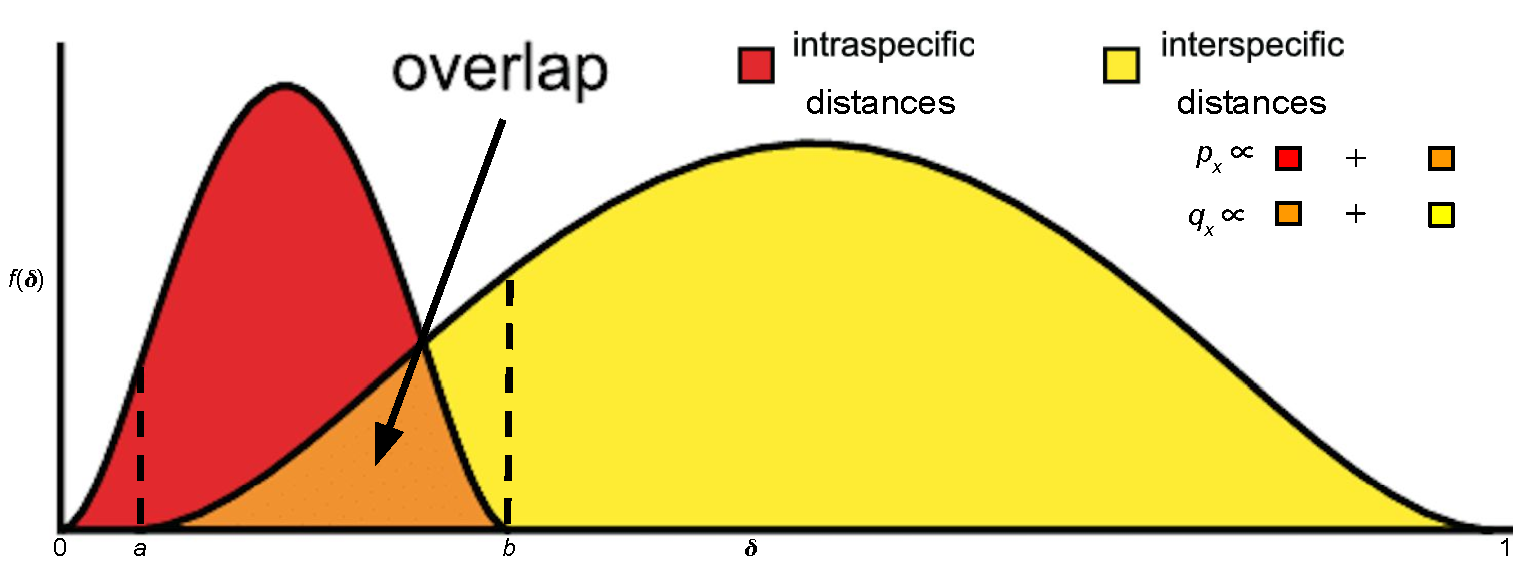
\includegraphics[width=1.0\textwidth]{Figure 1}

\caption{Modified depiction from \citet{meyer2005dna} and \citet{phillips2024measure} of the overlap/separation of pairwise intraspecific and interspecific pairwise genetic distances ($\delta$) for calculation of the DNA barcode gap metrics ($p_x$ and $q_x$) for a hypothetical species $x$. The minimum interspecific distance is denoted by $a$ and the maximum intraspecific distance is indicated by $b$. The quantity $f(\delta)$ is akin to a kernel density estimate of the probability density function of pairwise genetic distances. A similar visualization can be displayed for $p^{'}_x$ and $q^{'}_x$ within the interval [$a'$, $b$].}

\end{figure}

\newpage

\begin{table}[htbp]
    \centering
    \small
    \caption{Interpretation of the DNA barcode gap estimators within [$a/a'$, $b$]}.
    \label{tab:parameters}
    \begin{tabular}{cp{0.7\linewidth}}
    \hline
    \textbf{Parameter} & \textbf{Explanation} \\
    \hline
    $p_x$/$p_{\text{lwr}}$ & When $p_{\text{lwr}}$ is close to 0 (1), it suggests that the probability of intraspecific (interspecific) distances being larger (smaller) than interspecific (intraspecific) distances is low (high) on average, while the probability of interspecific (intraspecific) distances being larger (smaller)  than intraspecific (interspecific) distances is high (low) on average; that is, there is (no) evidence for a DNA barcode gap.\\
        & \\[-2mm]
     $q_x$/$p_{\text{upr}}$ & When $p_{\text{upr}}$ is close to 0 (1), it suggests that the probability of interspecific (intraspecific) distances being larger (smaller) than intraspecific (interspecific) distances is high (low) on average, while the probability of intraspecific (interspecific) distances being larger (smaaler) than interspecific (intraspecfic) distances is low (high) on average; that is, there is (no) evidence for a DNA barcode gap. \\
        & \\[-2mm]
    $p^{'}_x$/$p^{'}_{\text{lwr}}$ & When $p^{'}_{\text{lwr}}$ is close to 0 (1), it suggests that the probability of intraspecific (combined interspecific distances for a target species and its nearest neighbour species) distances being larger than combined interspecific distances for a target species and its nearest neighbour species (intraspecific distances) is low (high) on average, while the probability of combined interspecific distances for a target species and its nearest neighbour species (intraspecfic distances) being larger than intraspecific distances (combined interspecific distances for a target species and its nearest neighbour species) is high (low) on average; that is, there is (no) evidence for a DNA barcode gap.\\
        & \\[-2mm]
     $q^{'}_x$/$p^{'}_{\text{upr}}$ & When $p^{'}_{\text{upr}}$ is close to 0 (1), it suggests that the probability of combined interspecific distances for a target species and its nearest neighbour species (intraspecific distances) being larger than intraspecific distances (combined interspecific distances for a target species and its nearest neighbour species) is high (low) on average, while the probability of intraspecific distances (combined interspecific distances for a target species and its nearest neighbour species) being larger than combined interspecific distances for a target species and its nearest neighbour species (intraspecific distances) is low (high) on average; that is, there is (no) evidence for a DNA barcode gap.\\
    \hline
    \end{tabular}
\end{table}

\newpage

\begin{figure}[H]

\centering

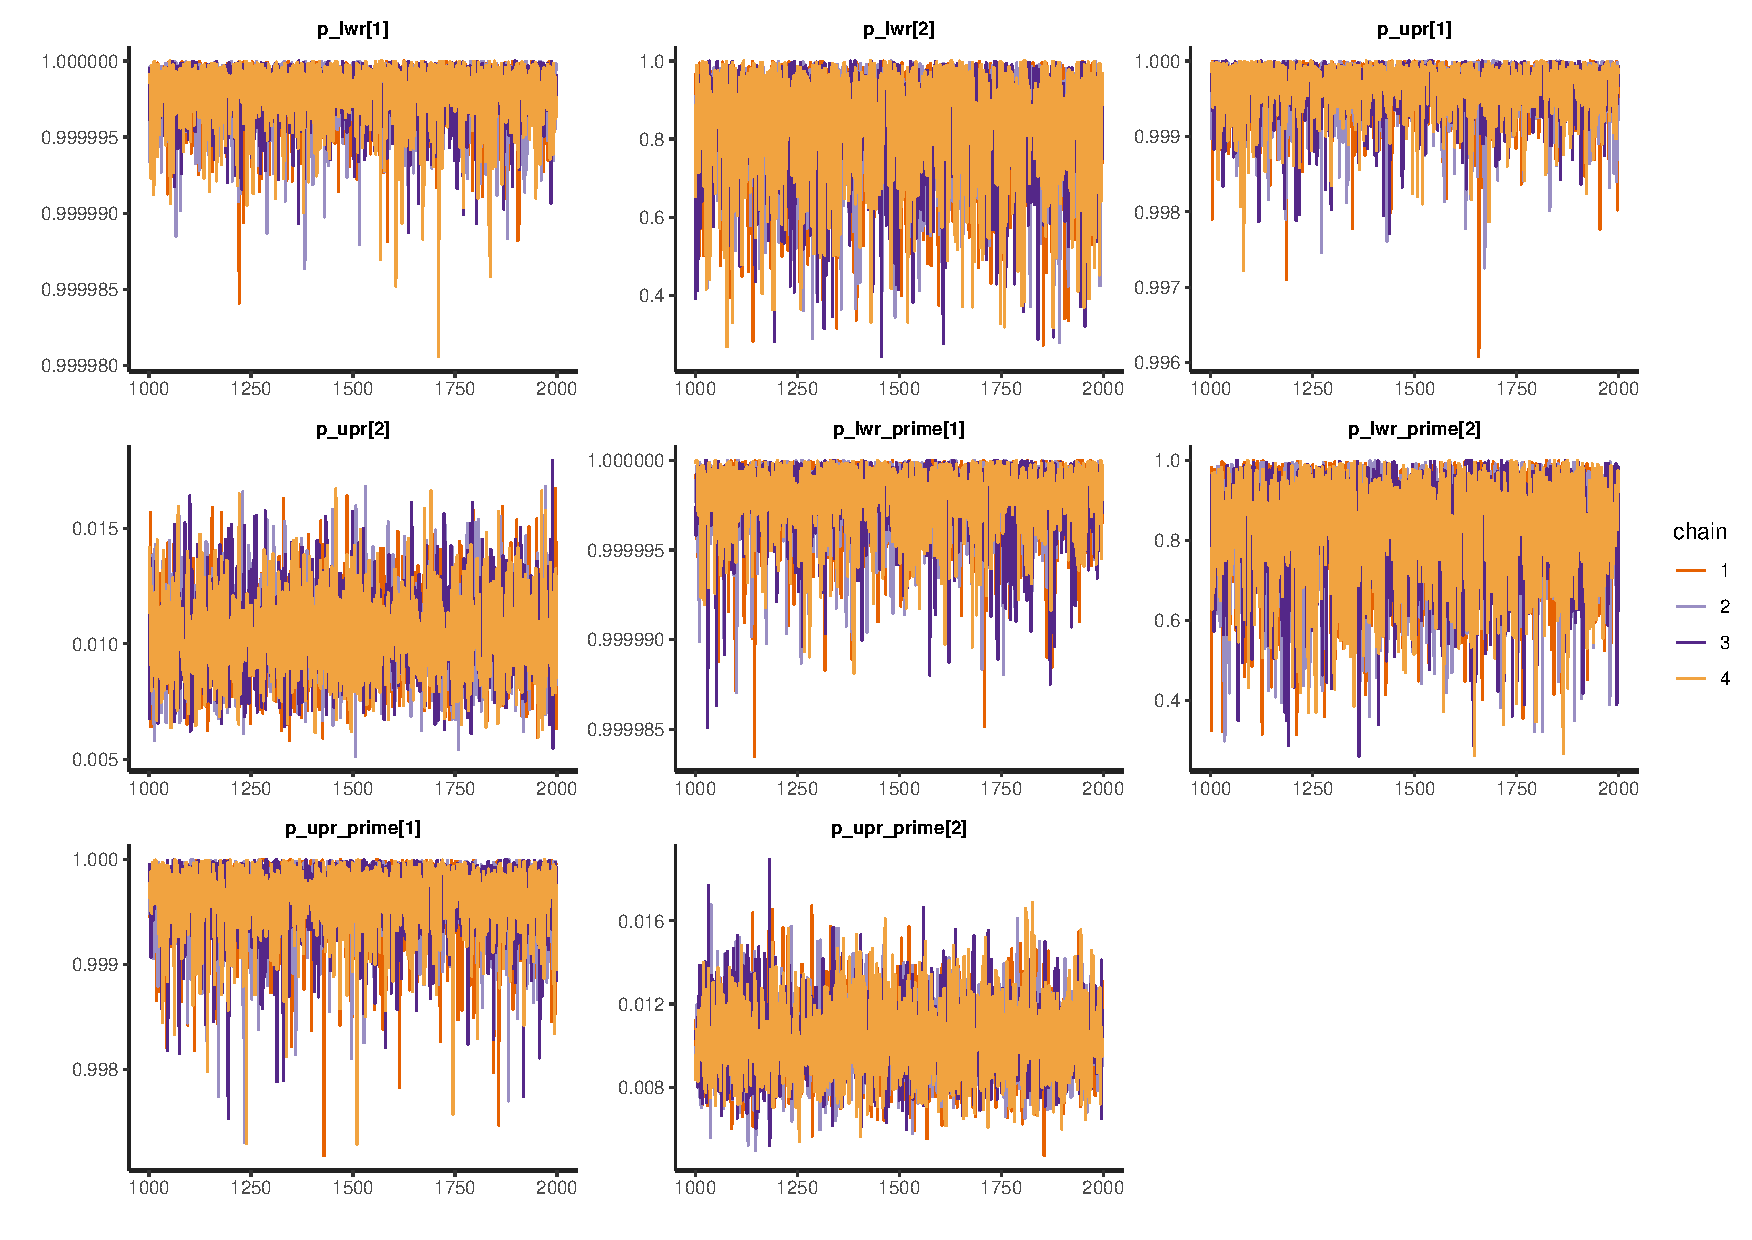
\includegraphics[width=0.80\textwidth]{Figure 2}

\caption{MCMC parameter traceplots applied to \textit{A. bipustulatus} ([1]; $n$ = 701) and \textit{A. nevadensis} ([2]; $n$ = 2) for CYTB across 1000 post-warmup iterations.}

\end{figure}

\newpage

\begin{landscape}
\begin{table}[H]

\centering

\caption{Nonparametric frequentist and Bayesian estimates of pairwise genetic distance distribution overlap/separation for the DNA barcode gap coalescent model parameters applied to \textit{A. bipustulatus} $n$ = 701) and \textit{A. nevadensis} $n$ = 2) for CYTB, including 95\%  CIs and CrIs. CrIs are based on 4000 posterior draws. All parameter estimates are reported to three decimal places of precision.}

\begin{tabular}{cccc} \hline

\textbf{Species} & \textbf{Parameter} & \textbf{MLE (SE, 95\% CI)} & \textbf{Bayes Est. (SD; 95\% CrI)} \\  \hline
\textit{A. bipustulatus} & $p_x/p_\mathrm{lwr}$ & 1.000 (0.000; 1.000-1.000) & 1.000 (0.000; 1.000-1.000) \\
\textit{A. bipustulatus} & $q_x/p_\mathrm{upr}$ & 1.000 (0.000; 1.000-1.000) & 1.000 (0.000; 0.999-1.000) \\
\textit{A. bipustulatus} & $p^{'}_x/p^{'}_\mathrm{lwr}$ & 1.000 (0.000; 1.000-1.000) & 1.000 (0.000; 1.000-1.000)  \\
\textit{A. bipustulatus} & $q^{'}_x/p^{'}_\mathrm{upr}$ & 1.000 (0.000; 1.000-1.000) & 1.000 (0.000; 0.999-1.000) \\


\textit{A. nevadensis} & $p_x/p_\mathrm{lwr}$ & 1.000 (0.000; 1.000-1.000) & 0.835 (0.144; 0.470-0.996) \\
\textit{A. nevadensis} & $q_x/p_\mathrm{upr}$ & 0.010 (0.002; 0.006-0.014) & 0.010 (0.002; 0.007-0.014) \\
\textit{A. nevadensis} &  $p^{'}_x/p^{'}_\mathrm{lwr}$ & 1.000 (0.000; 1.000-1.000) & 0.834 (0.138; 0.481-0.994) \\
\textit{A. nevadensis} &  $q^{'}_x/q^{'}_\mathrm{upr}$ & 0.010 (0.070; -0.128-0.148) & 0.010 (0.002; 0.007-0.014) \\


\hline


\end{tabular}

\end{table}
\end{landscape}

\newpage

\begin{landscape}
\begin{table}[H]

\centering

\caption{Posterior Predictive Checks of pairwise genetic distance distribution overlap/separation for the DNA barcode gap coalescent model parameters applied to \textit{A. bipustulatus} $n$ = 701) and \textit{A. nevadensis} $n$ = 2) for CYTB. CrIs are based on 4000 posterior draws. All parameter estimates are reported to three decimal places of precision.}

\begin{tabular}{ccccc} \hline

\textbf{Species} & \textbf{Variable} & $\textbf{\textit{Y}}$ & $\textbf{\textit{n}}$ & \textbf{Bayes Est. (SD; 95\% CrI)} \\  \hline

\textit{A. bipustulatus} & $y_\mathrm{lwr}$ & 491401.000 & 491401.000 & 491400.018 (1.378, 491396.000-491401.000) \\
\textit{A. bipustulatus} & $y_\mathrm{upr}$ & 2804.000 & 2804.000 & 2803.019 (1.433, 2799.000-2804.000) \\
\textit{A. bipustulatus} & $y^{'}_\mathrm{lwr}$ & 491401.000 & 491401.000 & 491400.008 (1.412, 491396.000-491401.000) \\
\textit{A. bipustulatus} & $y^{'}_\mathrm{upr}$ & 2804.000 & 2804.000 & 2802.992 (1.429, 2799.000-2804.000) \\

\textit{A. nevadensis} & $y_\mathrm{lwr}$ & 4.000 & 4.000 & 3.355 (0.888, 1.000-4.000) \\
\textit{A. nevadensis} & $y_\mathrm{upr}$ & 28.000 & 2804.000 & 29.151 (7.620, 16.000-45.000) \\
\textit{A. nevadensis} & $y^{'}_\mathrm{lwr}$ & 4.000 & 4.000 & 3.325 (1.000-4.000) \\
\textit{A. nevadensis} & $y^{'}_\mathrm{upr}$ & 28.000 & 2804.000 & 28.942 (15.000-45.000)  \\


\hline


\end{tabular}

\end{table}
\end{landscape}

\newpage

\begin{figure}[H]

\centering

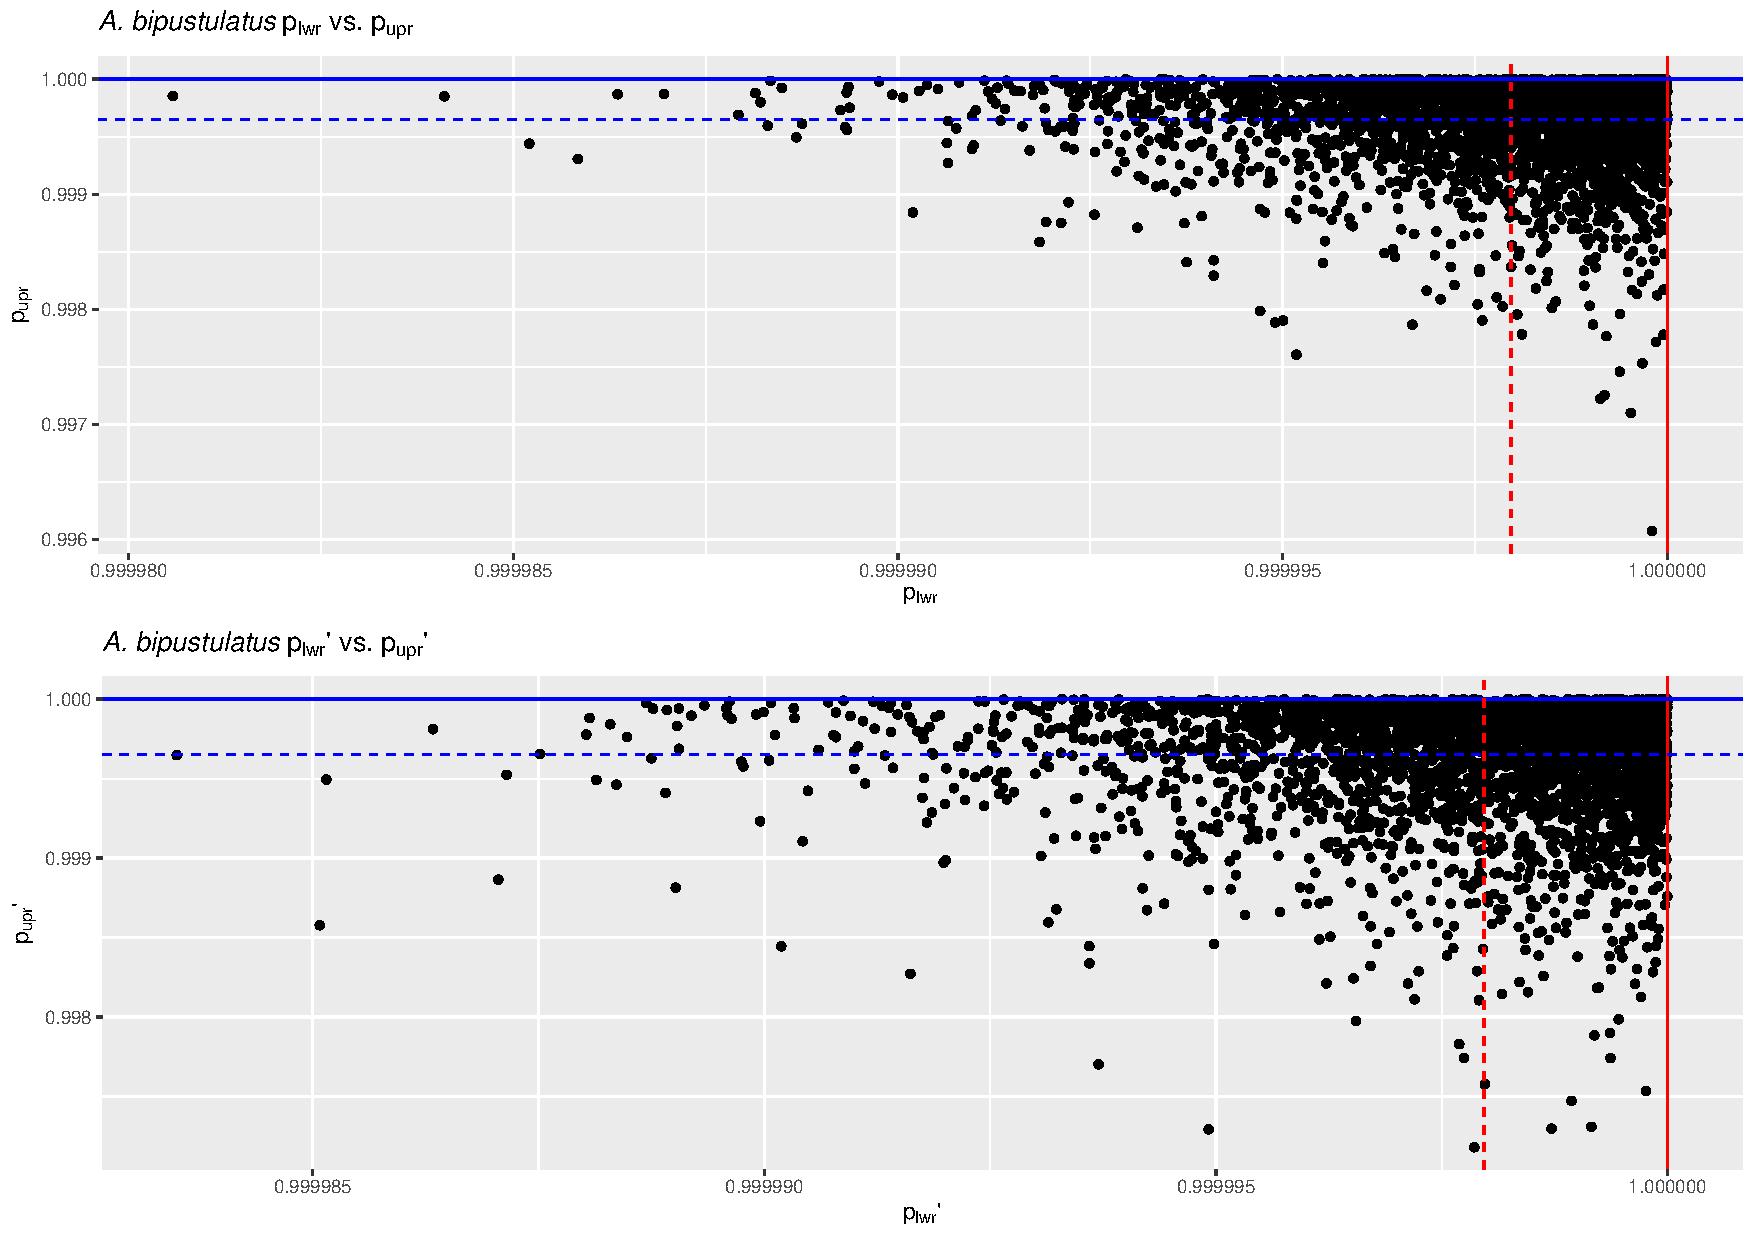
\includegraphics[width=0.80\textwidth]{Figure 3}

\caption{Scatterplot of Bayesian posterior draws ($n$ = 4000; black solid points) for \textit{A. bipustulatus} ($n$ = 701) across CYTB. MLEs and posterior means are displayed as coloured (red/blue) solid and dashed lines for the metrics, respectively.}

\end{figure}

\newpage


\begin{figure}[H]

\centering

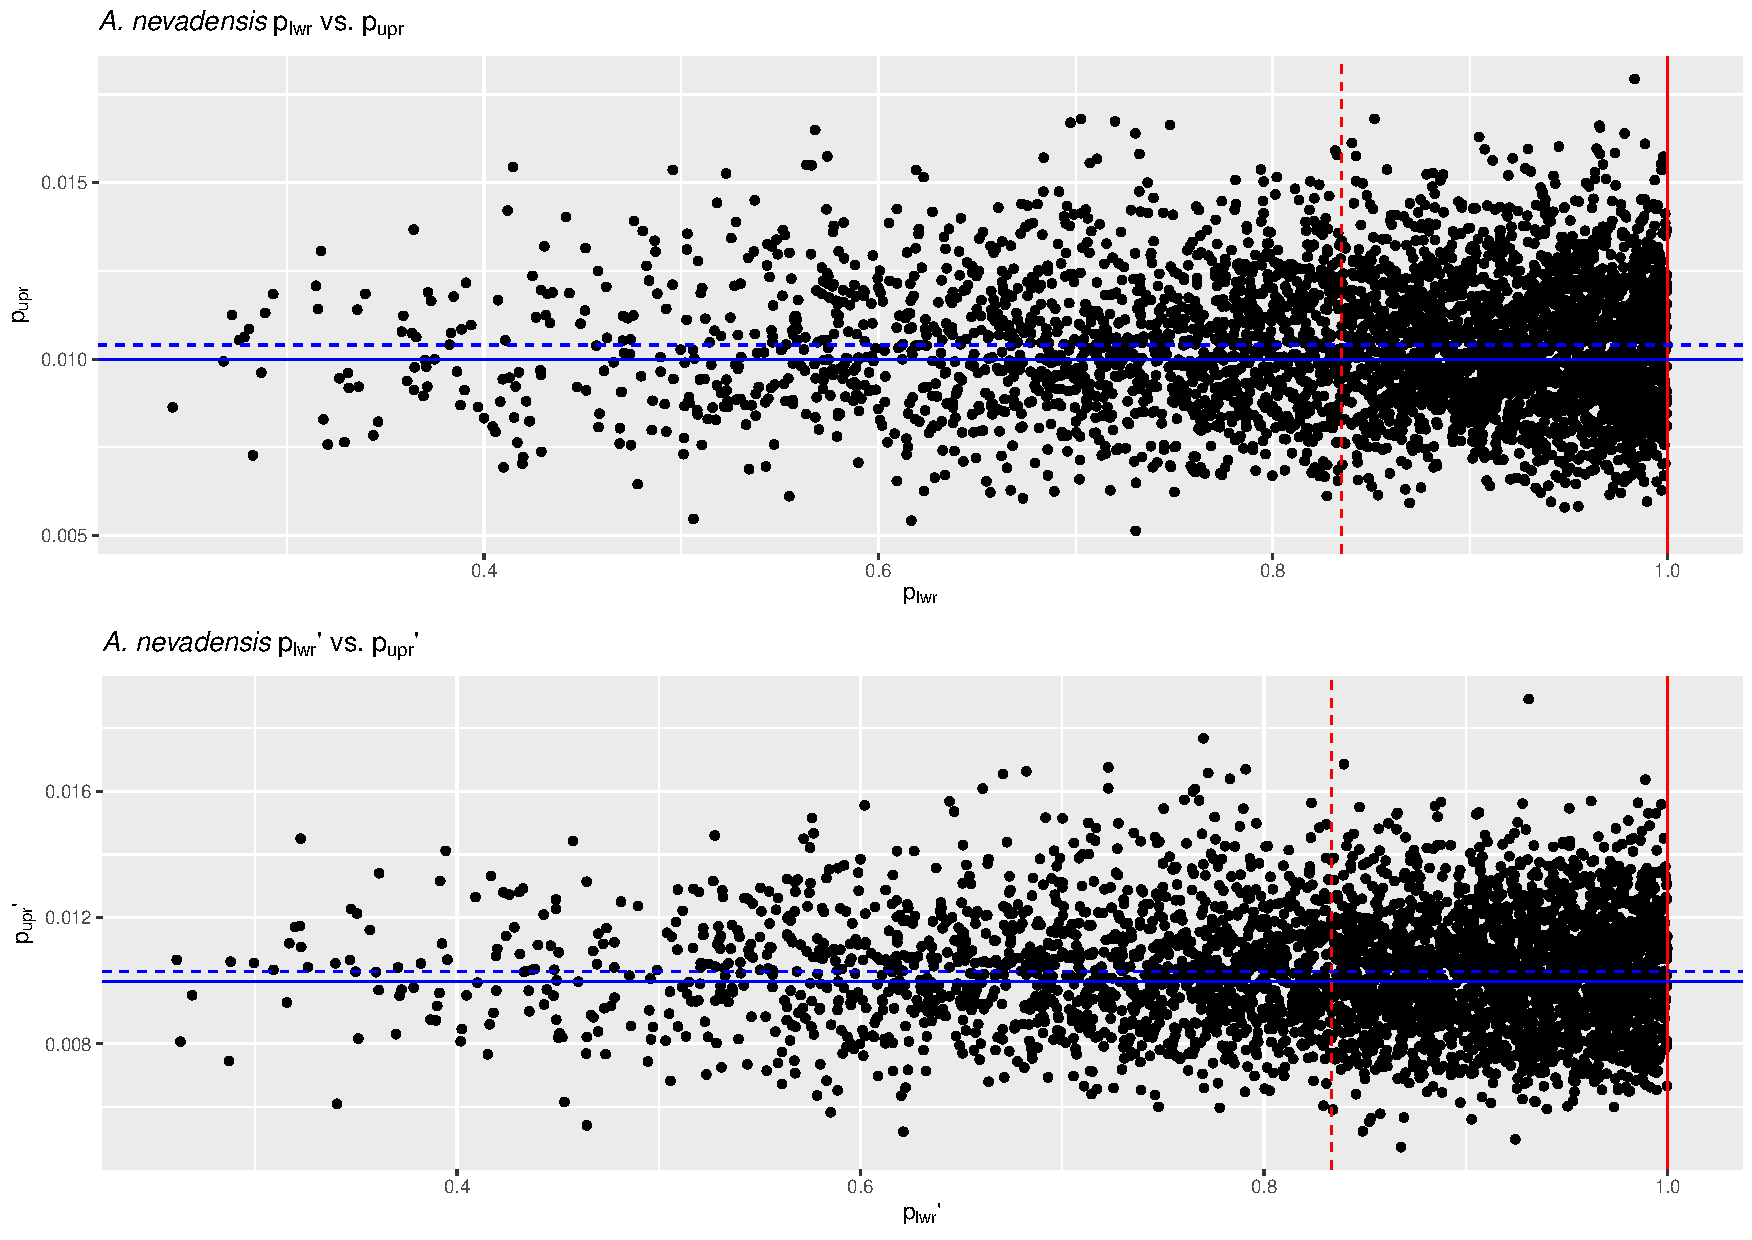
\includegraphics[width=0.80\textwidth]{Figure 4}

\caption{Scatterplot of Bayesian posterior draws ($n$ = 4000; black solid points) for \textit{A. nevadensis} ($n$ = 2) across CYTB. MLEs and posterior means are displayed as coloured (red/blue) solid and dashed lines for the metrics, respectively.}

\end{figure}

\newpage


\begin{figure}[H]

\centering

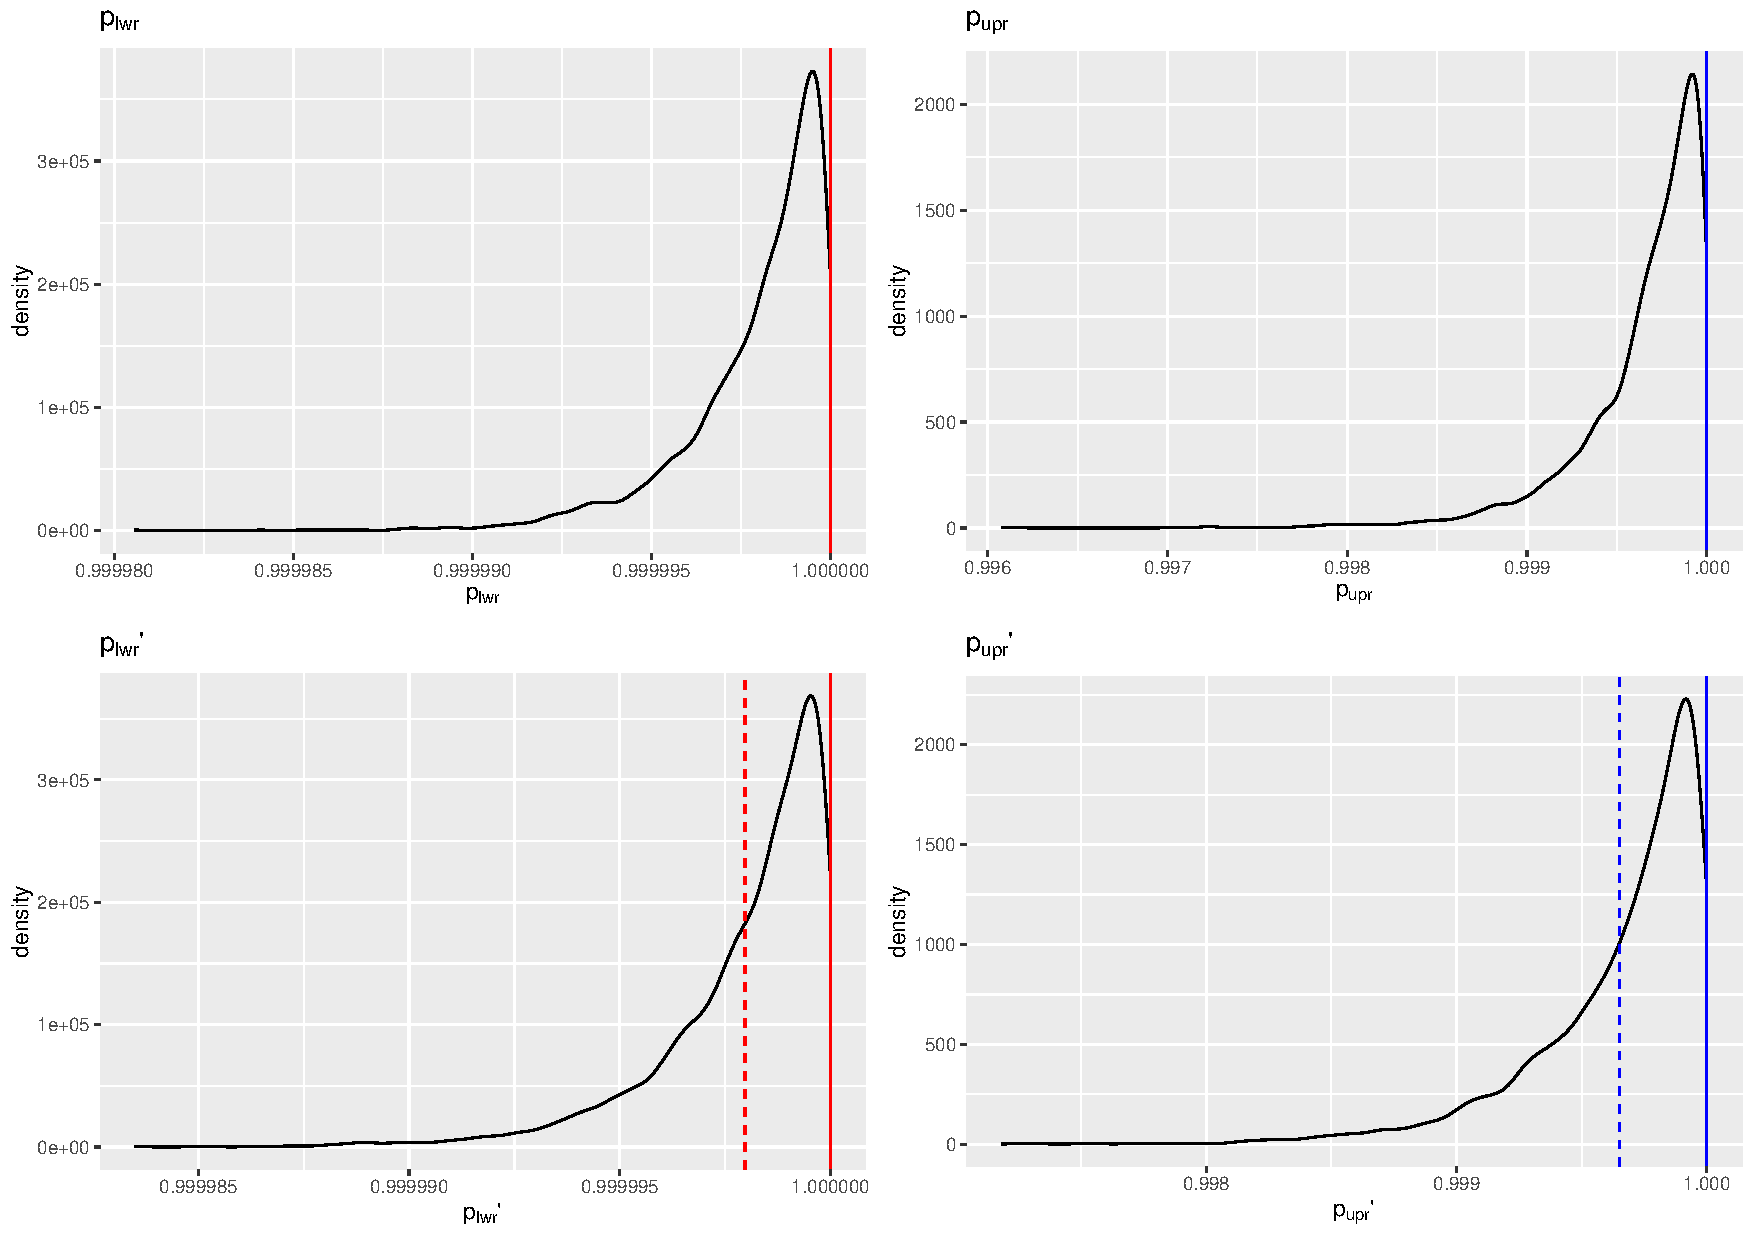
\includegraphics[width=0.80\textwidth]{Figure 5}

\caption{Posterior distributions based on 4000 draws of the DNA barcode gap metrics depicted as density plots for \textit{A. bipustulatus}. MLEs and posterior means are displayed as coloured (red/blue) solid and dashed lines for the metrics, respectively.}

\end{figure}

\newpage


\begin{figure}[H]

\centering

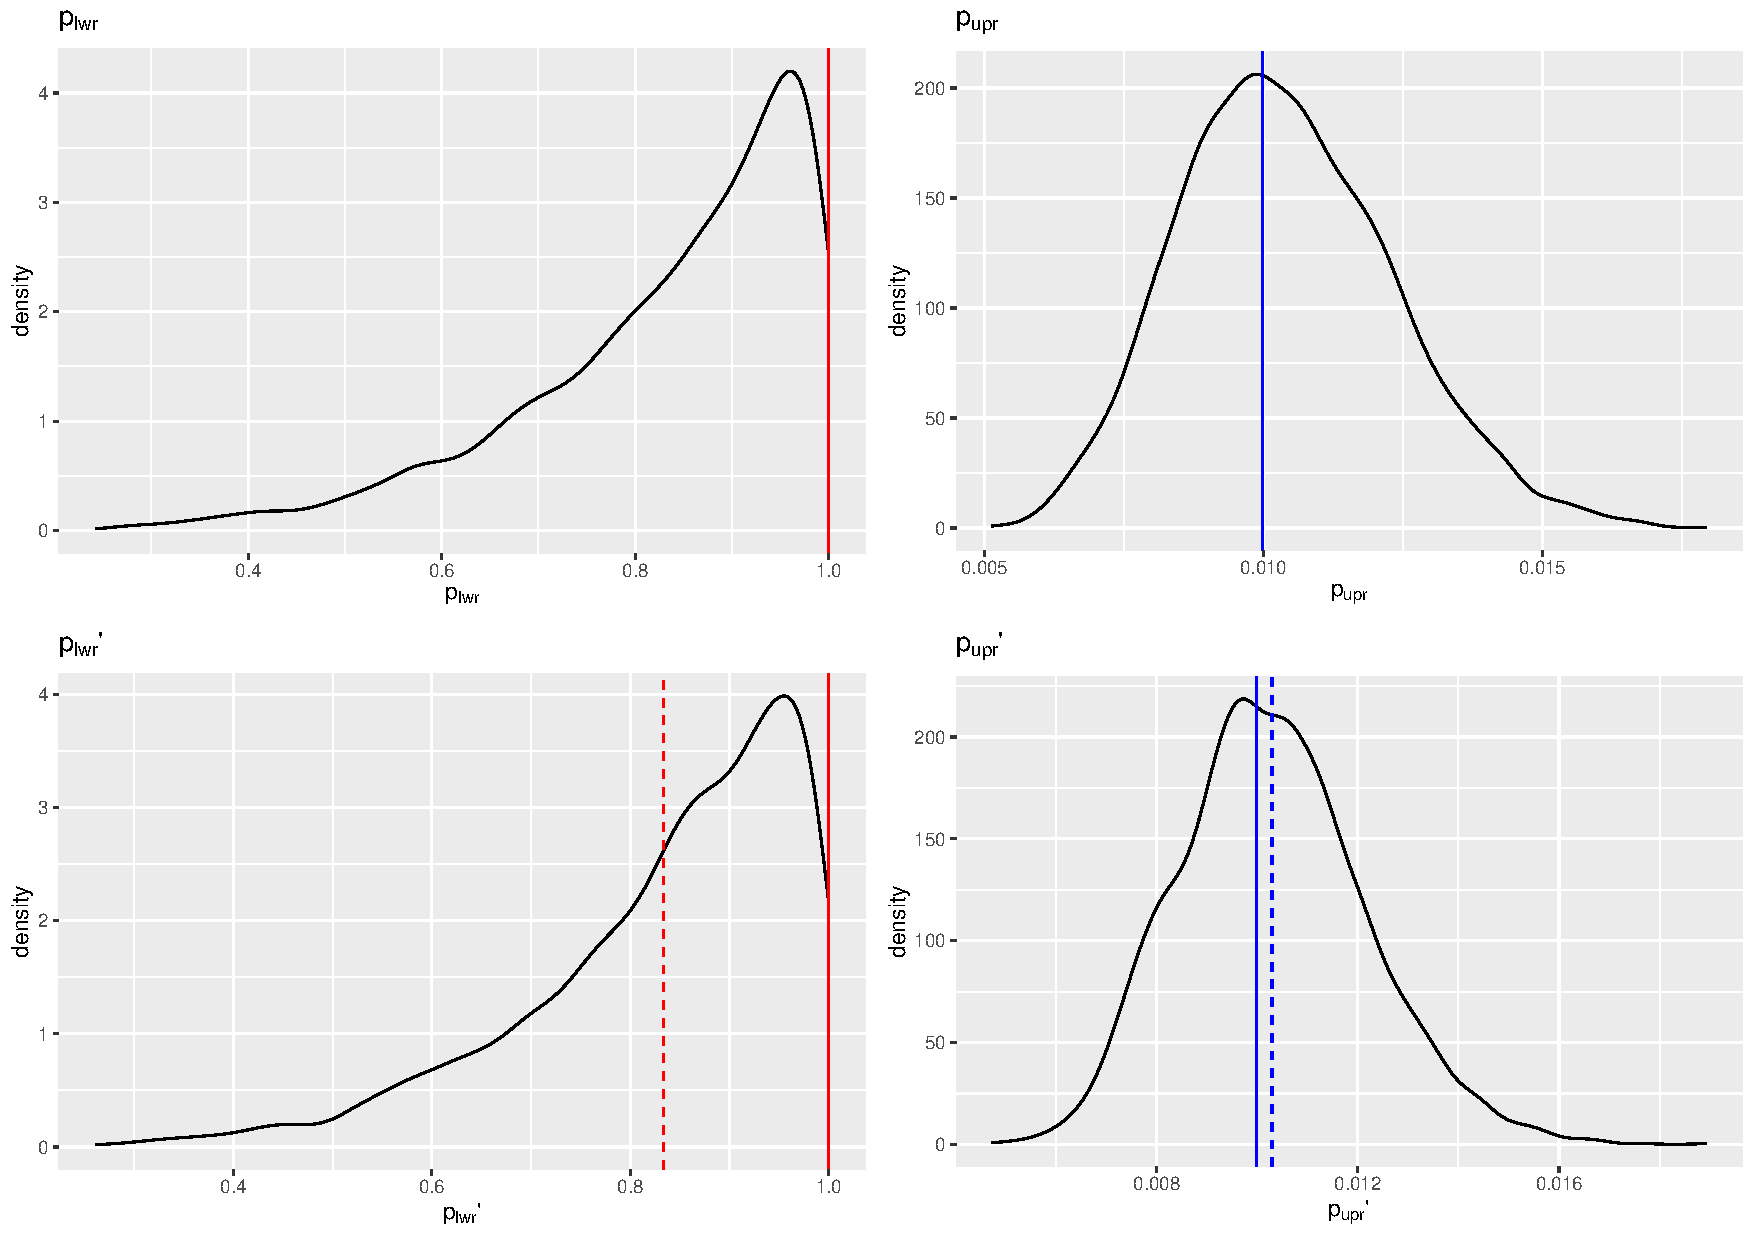
\includegraphics[width=0.80\textwidth]{Figure 6}

\caption{Posterior distributions based on 4000 draws of the DNA barcode gap metrics depicted as density plots for \textit{A. nevadensis}. MLEs and posterior means are displayed as coloured (red/blue) solid and dashed lines for the metrics, respectively.}

\end{figure}

\end{document}